\documentclass[aspectratio=169,xcolor=dvipsnames]{beamer}
\usetheme{SimplePlus}

\usepackage{hyperref}
\usepackage{graphicx} % Allows including images
\usepackage{booktabs} % Allows the use of \toprule, \midrule and \bottomrule in tables

\title{Nobel Ontology}
\subtitle{Group A3D}

\author{Andrea Bruttomesso, Alessandro Corr\`o, Davide Seghetto, Andrea Stocco}

\date{January 15, 2025} % Date, can be changed to a custom date

\setbeamertemplate{footline}{\leavevmode%
\begin{beamercolorbox}[wd=.33\paperwidth,left,ht=2.5ex,dp=1.5ex,leftskip=0.5ex]{subsection in head/foot} A3D
\end{beamercolorbox}%
\begin{beamercolorbox}[wd=.33\paperwidth,center,ht=2.5ex,dp=1.5ex]{section in head/foot}
  \usebeamercolor[fg]{section in foot/head}\insertshorttitle
\end{beamercolorbox}%
\begin{beamercolorbox}[wd=.34\paperwidth,right,ht=2.5ex,dp=1.5ex, rightskip=1.5ex]{subsection in head/foot}
  \insertshortdate
\end{beamercolorbox}%
}

%----------------------------------------------------------------------------------------
%    PRESENTATION SLIDES
%----------------------------------------------------------------------------------------
\begin{document}

\begin{frame}
	% Print the title page as the first slide
	\titlepage
\end{frame}

\begin{frame}{Overview}
	% Throughout your presentation, if you choose to use \section{} and \subsection{} commands, these will automatically be printed on this slide as an overview of your presentation
	\tableofcontents
\end{frame}

\section{Domain of Interest}

\begin{frame}{Domain of Interest}
	\centering
	\begin{minipage}{0.3\textwidth}
		\centering
		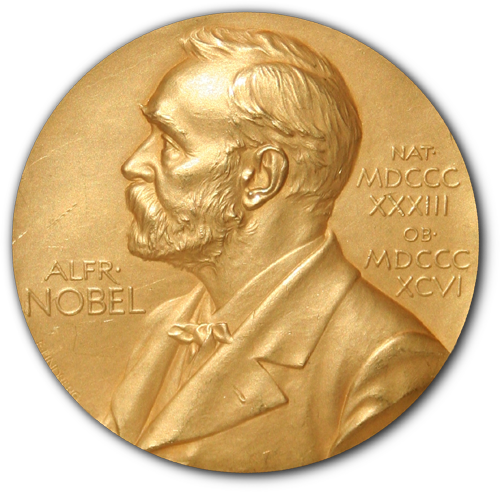
\includegraphics[width=\textwidth]{nobel.png} % Left image
	\end{minipage}%
	\hspace{3em}
	\begin{minipage}{0.4\textwidth}
		\centering
		We have chosen the domain of scientific research. Specifically, we aim to analyze potential correlations among Nobel Prize winners,
		their publications, and the research funding invested by various countries. This domain was selected because it allows us to reveal potential historical
		and geographical patterns in scientific research.
	\end{minipage}%
\end{frame}

\section{Ontology Design}

\begin{frame}
	\begin{figure}
		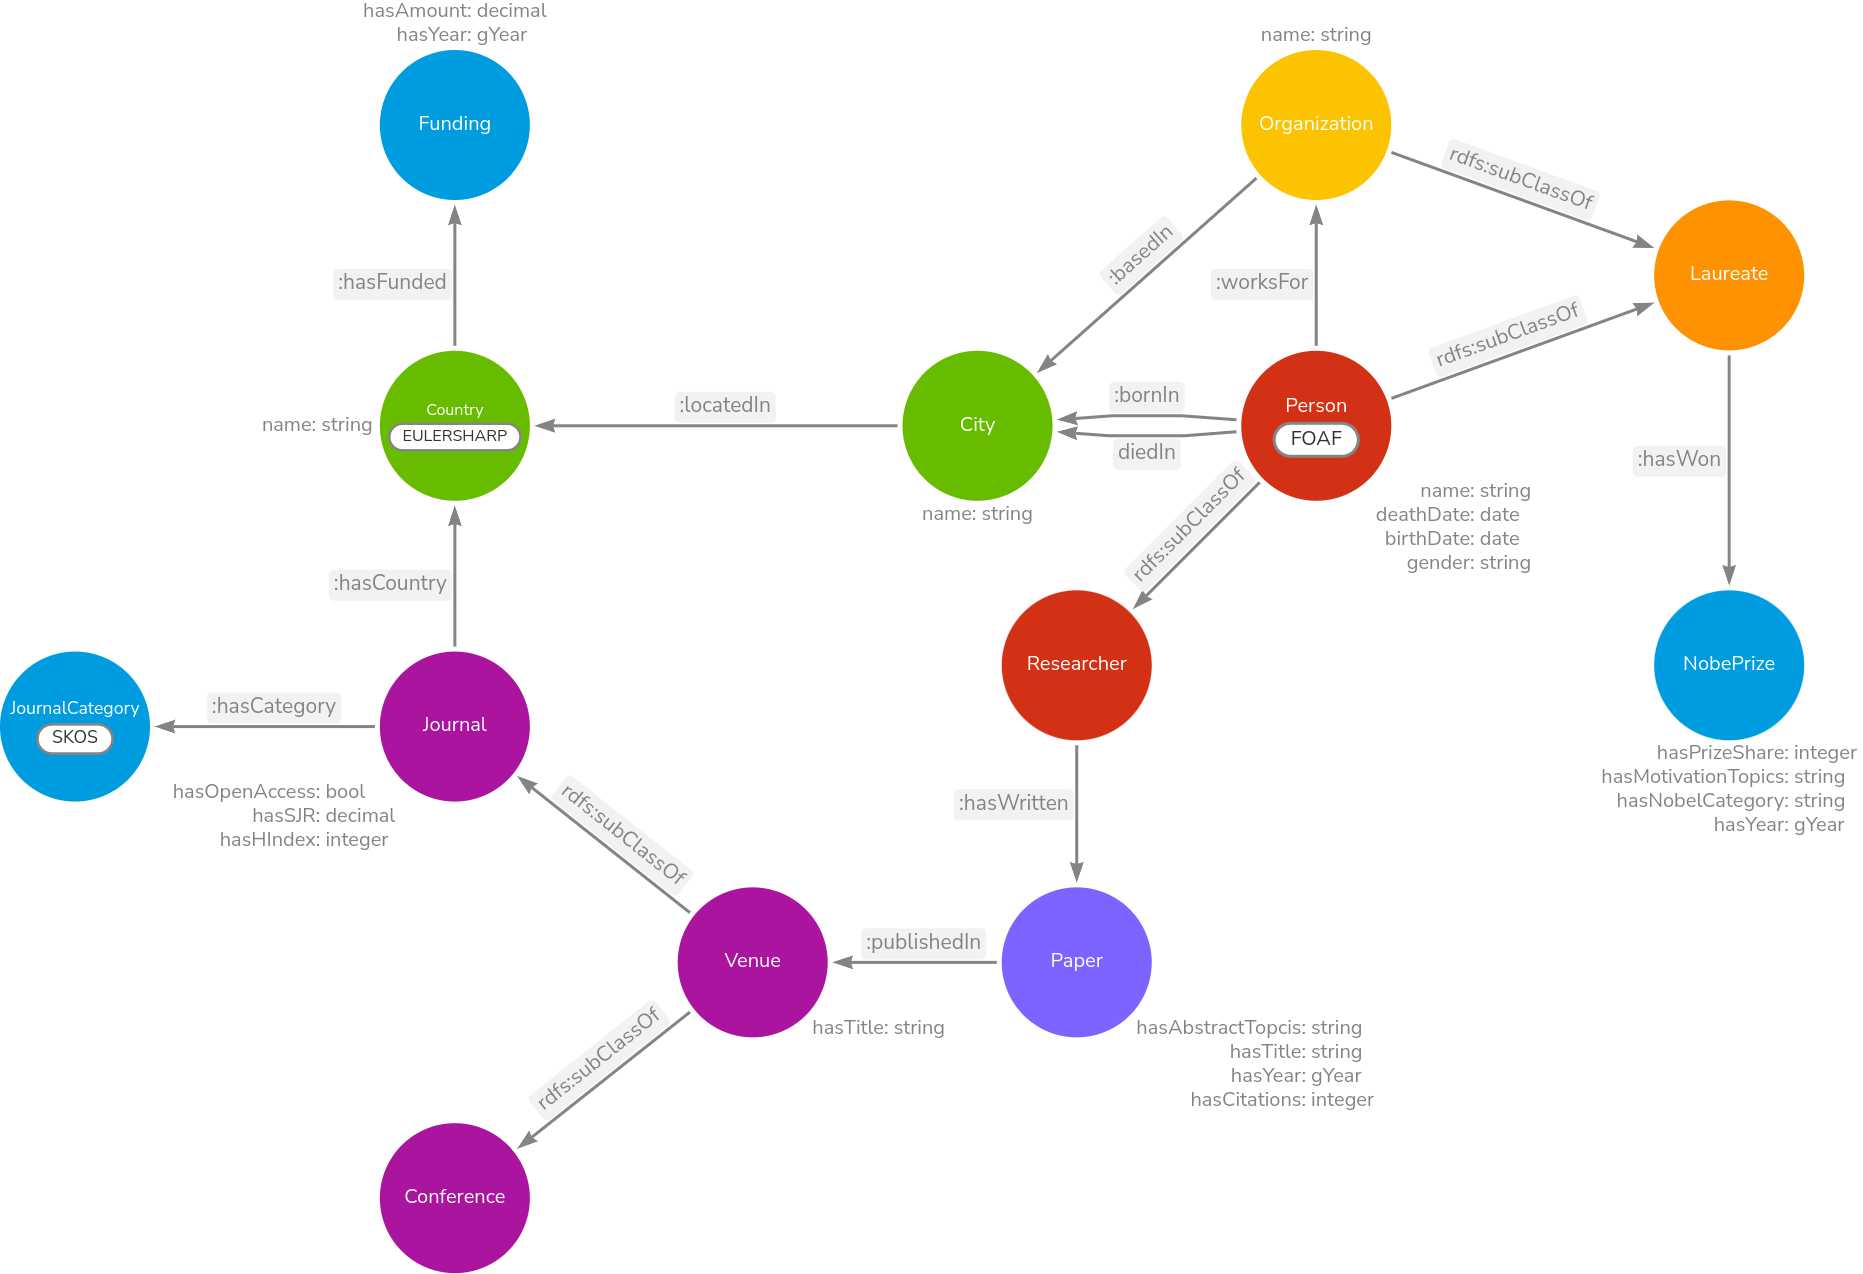
\includegraphics[width=0.75\linewidth]{../nobelOntologyTransparent.png}
	\end{figure}
\end{frame}

\section{Challenges}

\begin{frame}{Challenges}
	\begin{itemize}
		\item Errors in Nobel Laureates dataset
		      \vspace{1em}
		\item Topic Modeling
		      \vspace{1em}
		\item Subset of papers dataset
		      \vspace{1em}
		\item Researchers and Nobel Laureates matching names
	\end{itemize}
\end{frame}

\begin{frame}{Errors in Nobel Laureate dataset}
	\begin{table}[H]
		\centering
		\caption{Example of dataset error}
		\resizebox{.6\linewidth}{!}{\begin{tabular}{|l|l|l|l|}
				\hline
				\textbf{Year} & \textbf{Category} & \textbf{Prize Share} & \textbf{Full Name}    \\ \hline
				1908          & Medicine          & 1/2                  & Ilya Ilyich Mechnikov \\ \hline
				1908          & Medicine          & 1/2                  & Paul Ehrlich          \\ \hline
				1908          & Medicine          & 1/2                  & Paul Ehrlich          \\ \hline
			\end{tabular}}
		\label{tab:datasetError}
	\end{table}
\end{frame}

\begin{frame}{Papers dataset was too big}
	\centering
	\begin{minipage}{0.8\textwidth}
		\centering
		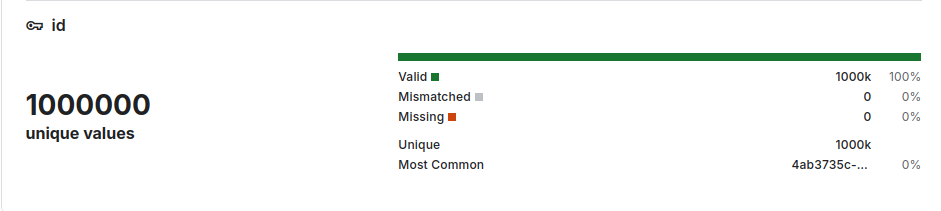
\includegraphics[width=0.9\textwidth]{huge_dataset.png}
	\end{minipage} \\
	\vspace{1em}
	\begin{minipage}{0.8\textwidth}
		The Papers Dataset originally contained 1 million rows, which made it necessary to filter the data.
		After careful consideration, we decided to retain only the papers authored by a Laureate or published
		in a venue included in the Venues Dataset.
		Even with this filter applied, the dataset still contained approximately 300,000 rows so we further
		reduced it by selecting only the first 50,000 rows.
	\end{minipage}
\end{frame}

\begin{frame}{Researchers and Nobel Laureates matching names}
	The Laureates and Papers Datasets often represent names differently, such as "Antoine Henri Becquerel"
	and "Antoine H. Becquerel." To effectively link these datasets, we utilized a library that implements a
	fuzzy matching algorithm with a similarity threshold of 90\%. This approach allowed us to identify and
	match names that were not identical but sufficiently similar, ensuring a robust connection between the
	datasets.
\end{frame}

\section{Analytics}

\begin{frame}{Relationship between funding allocated for R\&D and possibility of winning a Nobel Prize}
	\begin{columns}[c]
		\column{0.65\textwidth}
		\begin{figure}[H]
			\centering
			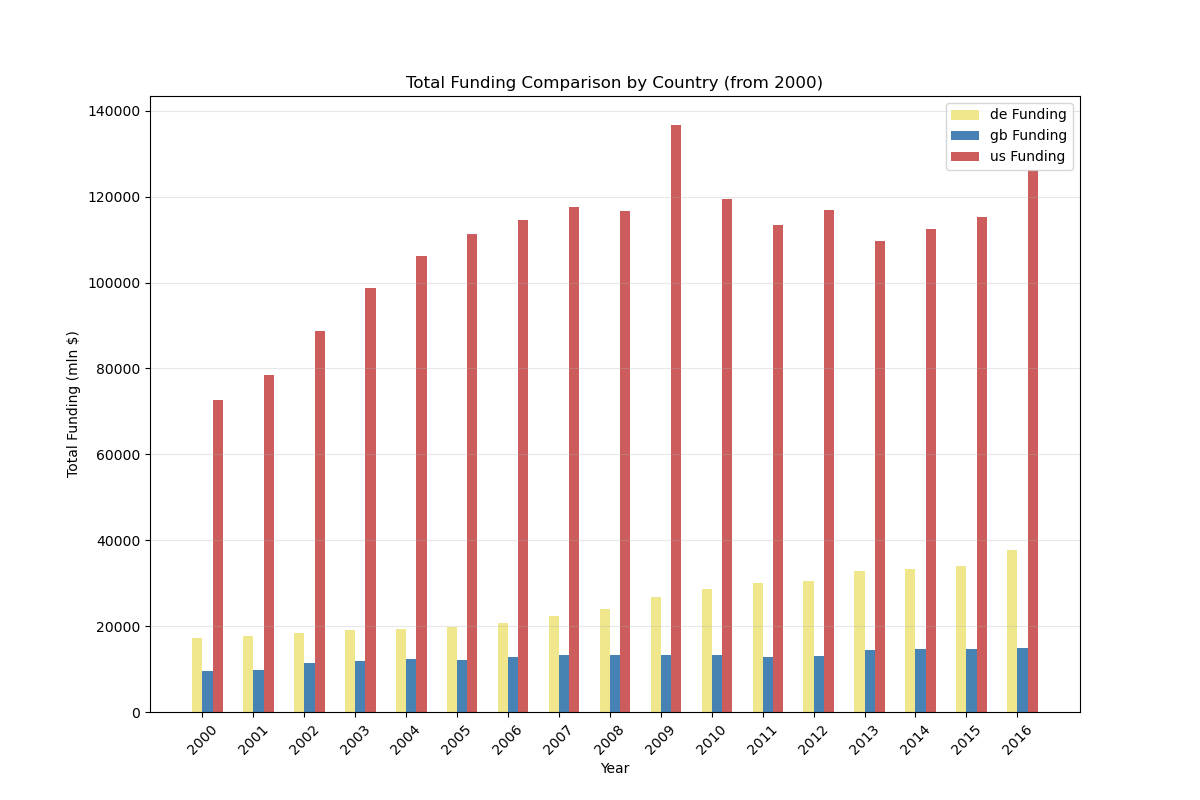
\includegraphics[width=\textwidth]{../queries/plots/funding_comparison_by_country.png}
			\label{fig:fundings_per_country}
		\end{figure}
		\column{0.35\textwidth}
		Germany's R\&D funding has been increasing over the years, whereas
		Great Britain's funding remains lower and more stable.
	\end{columns}
\end{frame}

\begin{frame}{Relationship between funding allocated for R\&D and possibility of winning a Nobel Prize (continued)}
	\begin{columns}[c]
		\column{0.65\textwidth}
		\begin{figure}[H]
			\centering
			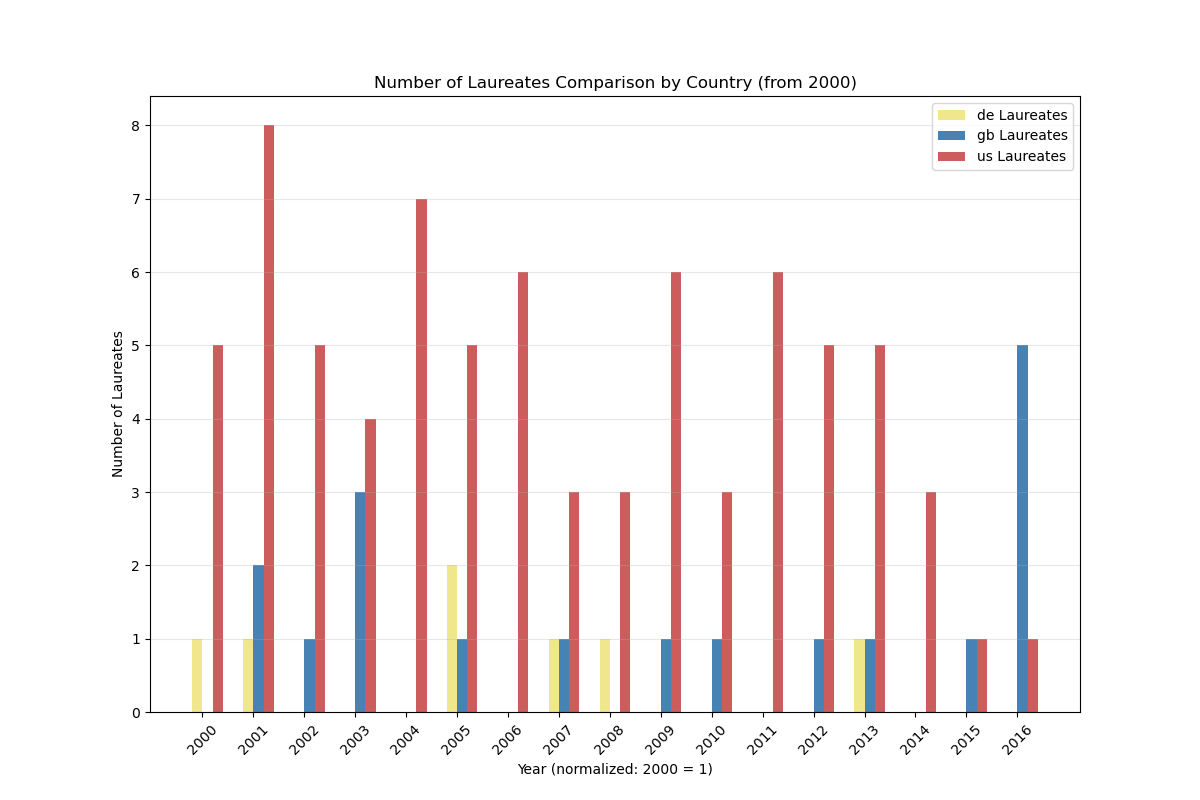
\includegraphics[width=\textwidth]{../queries/plots/laureates_comparison_by_country.png}
			\label{fig:laureates_per_country}
		\end{figure}
		\column{0.35\textwidth}
		These two plots suggest that the link between funding and Nobel prizes is not always
		straightforward.
	\end{columns}
\end{frame}

\begin{frame}{Nobel laureates: birthplace vs. research location by state}
	\begin{table}[h!]
		\centering
		\caption{States with lowest percentage of Laureates active in their home country}
		\begin{tabular}{|c|c|c|c|c|}
			\hline
			\textbf{State} & \textbf{Laureates} & \textbf{Laureates active in their home country} & \textbf{Percentage} \\ \hline
			Canada         & 19                 & 2                                               & 10,5\%              \\ \hline
			China          & 11                 & 2                                               & 18,2\%              \\ \hline
			Italy          & 19                 & 4                                               & 21\%                \\ \hline
			Austria        & 17                 & 4                                               & 23,5\%              \\ \hline
			Australia      & 11                 & 3                                               & 27,3\%              \\ \hline
		\end{tabular}
		\label{tab:laureates_active}
	\end{table}

	\textbf{Interesting insight:} Japan, despite being the seventh country in terms of Nobel
Prizes won, manages to retain nearly 67\% of its laureates within its borders. On the other hand, Russia, despite
being the sixth country in terms of Nobel Prizes won, has a retention rate of only 35\%.

\end{frame}

\begin{frame}{Nobel laureates: birthplace vs. research location by state}
	\begin{figure}[H]
		\centering
		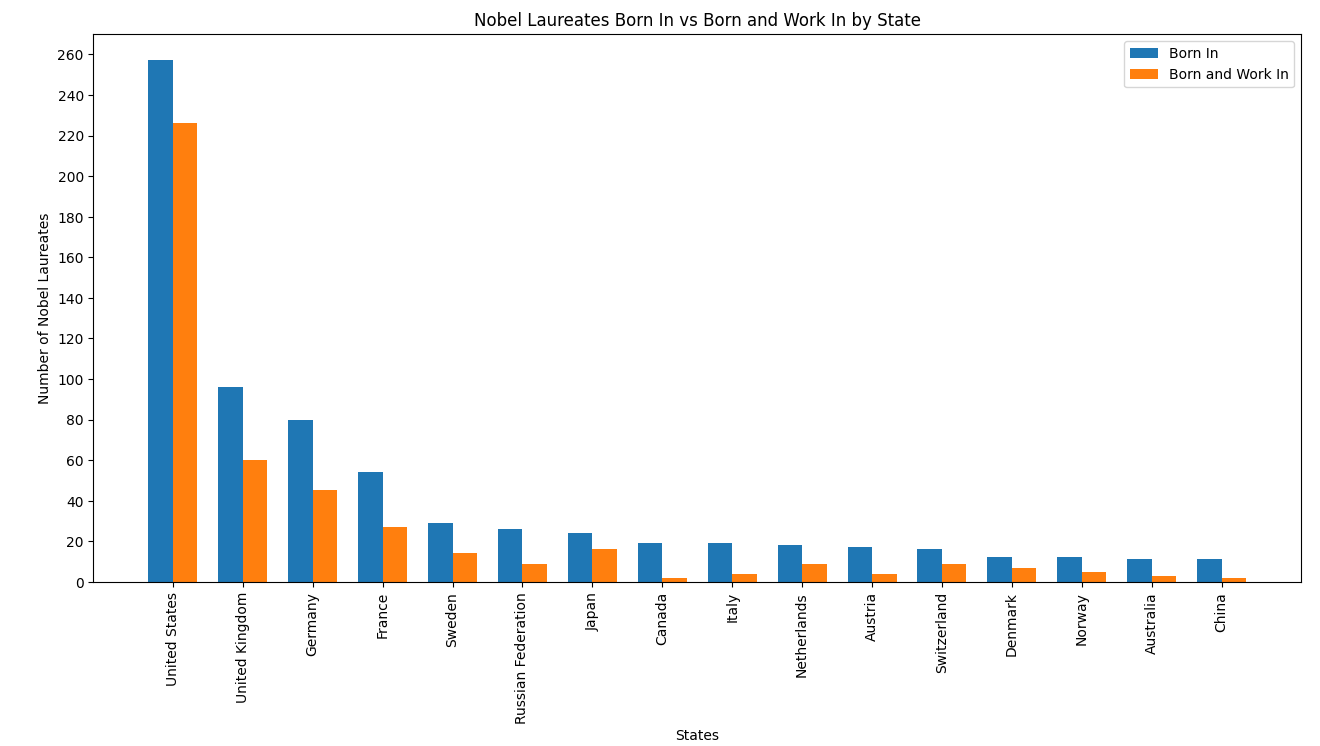
\includegraphics[width=0.75\textwidth]{../queries/plots/laureatesComparison.png}
		\caption{Comparison between Laureates who stayed in their home country and those who moved abroad}
		\label{fig:laureatesComparison}
	\end{figure}
\end{frame}

\begin{frame}{Age analysis of Nobel Prize winners}
	\begin{table}[H]
		\centering
		\caption{Age statistics of Nobel Prize winners by category}
		\begin{tabular}{|l|c|c|c|}
			\hline
			\textbf{Category} & \textbf{Min Age} & \textbf{Avg Age} & \textbf{Max Age} \\ \hline
			Chemistry         & 35               & 58               & 85               \\ \hline
			Economics         & 51               & 67               & 90               \\ \hline
			Literature        & 42               & 65               & 88               \\ \hline
			Medicine          & 32               & 58               & 87               \\ \hline
			Peace             & 17               & 61               & 87               \\ \hline
			Physics           & 25               & 55               & 88               \\ \hline
		\end{tabular}
		\label{tab:age_analysis}
	\end{table}

	\begin{footnotesize} % Puoi usare anche \scriptsize o \tiny per ridurre ulteriormente
		\begin{itemize}
			\item \textbf{Economics}: This category has the highest average age, with the eldest being Leonid Hurwicz.
		
			\item \textbf{Peace}: This category includes the youngest laureate, who is Malala Yousafzai at only 17 years old.
		
			\item \textbf{Chemistry, Medicine, and Physics}: These science-related categories show the lowest average and minimum age.
		
			\item \textbf{Literature}: This category has a high average age due also to the recognition of an author's entire career.
		\end{itemize}
		\end{footnotesize}
\end{frame}

\begin{frame}
	\Huge{\centerline{\textbf{Questions?}}}
\end{frame}

\end{document}
